\section{Integrationstest}
Integrationstests udføres for at checke om de enkelte software moduler passer sammen. Helt konkret drejer det sig om at finde de komponenter der forårsager \textit{Intercomponent failures}. De fleste interoperability fejl findes ikke med komponent scope testing Det er vigtigt at teste dette før der testes i \textit{system scope}.\\

I OO programmering kan integrationstest forgå løbende. Med dette menes at der kan foretages integrationstest for hver iteration. \\

Måden hvorpå en integrationstest adskiller sig fra en unittest er ved at den ikke er konsistent og/eller har en eller flere \textit{rigtige} afhængigheder. En test der fx afhænger af DateTime, er ikke længere kosnistent idet tiden ændrer sig for hver test.

\subsection{Forarbejde og strategi}\\

\begin{itemize}
	\item Hvilke komponenter er i fokus?
	\item I hvilken rækkefølge skal komponenterne testes?
	\item Hvilken test design teknik skal bruge?
\end{itemize}

Før man begynder at integrationsteste er der nogle ting som man bør have opfyldt:

\begin{itemize}
	\item Unittests skal være færdige. Dette gælder for samtlige metoder!
	\item Systemets dependancy tree skal være kendt! jf. ATM opgaven.
	\item Integrationstesten er planlagt.
\end{itemize}

\subsection{Typer af integrationstest}
Der findes flere typer af tilgange til at integrationsteste.

\subsubsection{Dependancy trees}
Dependancy trees er en måde at visualisere afhængighederne i et projekt. Det er vigtigt at have et overblik over sine dependancies når man skal planlægge integrationstest. På figur~\ref{fig:dependancyATM} vises et uddrag fra ATM opgavens dependancy tree.

\subsubsection{Drivers}
En driver er en klasse, eller et program der påtrykker testcases på den komponenten under test.

\begin{figure}[H]
\centering
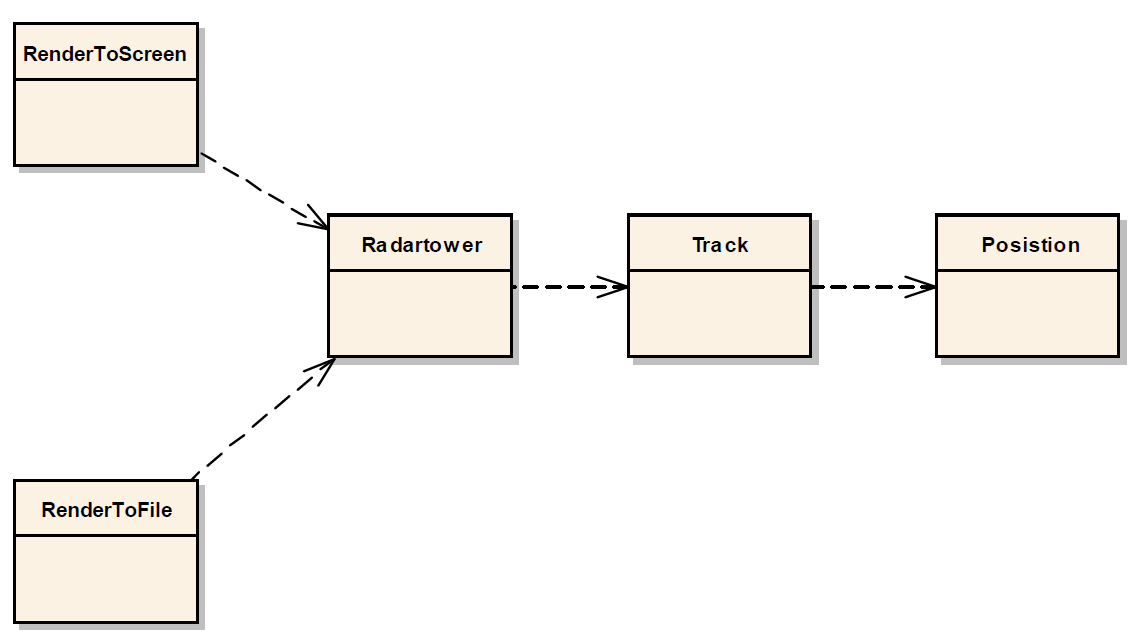
\includegraphics[width=0.78\linewidth]{figs/dependancyATM.PNG}
\caption{Uddrag fra ATM's dependancy model}
\label{fig:dependancyATM}
\end{figure}

Dependancy træet er opbygget så høj niveau modulerne ligger i den ene ende og lav niveau modulerne i den anden ende.

%%%%%%%%%%%%%%%%%%%%%%%%%%%%%%%%%%%%%%%%%%%%%%%%%%%%%%%%%%%%%%%%%%%%%%%%%%%%%%%%%%%%%%%%%%%%%%%%%%

\subsubsection{Big Bang testing}
I en \textit{Big Bang} integrationstest, sammensættes alle software komponenter, så det komplette system dannes. Herefter testes systemet.

\paragraph{Fordele Big Bang testing}
\begin{itemize}
	\item Man slipper for at planlægge sin test
	\item Nemt at bruge i mindre systemer
\end{itemize}

\paragraph{Ulemper ved Big Bang testing}
Der er en del ulemper ved denne integratoinstest model.

\begin{itemize}
	\item Man finder først fejlene når alle komponenter sættes sammen.
	\item Det er svært at isolere de fundne fejl.
	\item Der er stor sansynlighed for at misse kritiske fejl, som senere kan vise sig. \todo{hvorfor det?}
	\item Det er svært at dække alle test scenarier uden at misse enkelte.
	\item Bugfixing er last-minute og er derfor ofte af dårlig kvalitet.
\end{itemize}

%%%%%%%%%%%%%%%%%%%%%%%%%%%%%%%%%%%%%%%%%%%%%%%%%%%%%%%%%%%%%%%%%%%%%%%%%%%%%%%%%%%%%%%%%%%%%%%%%%

\subsubsection{Bottom-Up testing}

\begin{itemize}
	\item Starter i bunden af dependancy træet - nederste lag testes først.
\end{itemize}

\begin{figure}
\centering
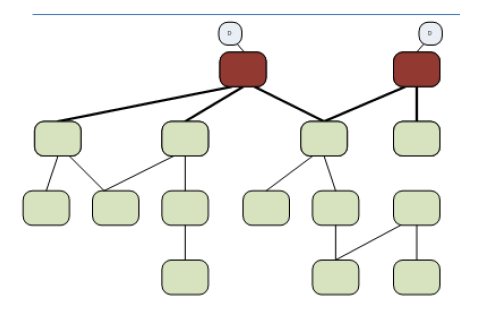
\includegraphics[width=0.7\linewidth]{figs/bottomUp.PNG}
\caption{Illustration af Bottom-Up testing.}
\label{fig:bottomUp}
\end{figure}

\paragraph{Fordele ved Bottom-Up testing}

\begin{itemize}
	\item Ingen eller få stubbe (Vi skal ikke fake dependancies).
	\item Let at dække interfaces på alle niveauer.
\end{itemize}

\paragraph{Ulemper ved Bottom-Up testing}

\begin{itemize}
	\item Kræver mange Drivere.
	\item Udsætter tests af kritiske kontrol interfaces.
\end{itemize}

%%%%%%%%%%%%%%%%%%%%%%%%%%%%%%%%%%%%%%%%%%%%%%%%%%%%%%%%%%%%%%%%%%%%%%%%%%%%%%%%%%%%%%%%%%%%%%%%%%

\subsubsection{Top-Down testing}

\begin{itemize}
	\item Starter i toppen af dependancy træet - øverste lag testes først.
\end{itemize}

\begin{figure}
\centering
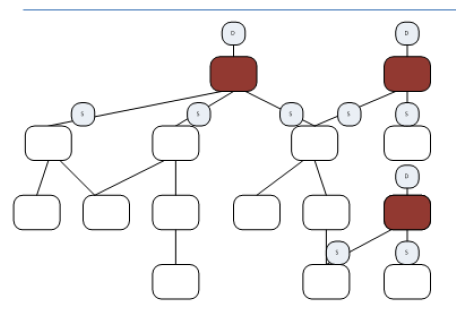
\includegraphics[width=0.7\linewidth]{figs/topDown.PNG}
\caption{Illustration af Top-Down testing.}
\label{fig:topDown}
\end{figure}

\paragraph{Fordele ved Top-Down testing}

\begin{itemize}
	\item Få Drivere skal skrives.
	\item Man udsætter ikke testing af kontrol komponenter.
	\item God til at arbejde samtidigt på HW og SW.
\end{itemize}

\paragraph{Ulemper ved Top-Down testing}

\begin{itemize}
	\item Bruger mange stubbe. Et isolation framework gør det dog lettere.
	\item Svært at repræsentere low-level interfaces i toppen. 
\end{itemize}

%%%%%%%%%%%%%%%%%%%%%%%%%%%%%%%%%%%%%%%%%%%%%%%%%%%%%%%%%%%%%%%%%%%%%%%%%%%%%%%%%%%%%%%%%%%%%%%%%%

\subsubsection{Collaboration testing}
Der vælges en "vej" gennem dependancy træet, fra top til bund. Eksempelvis en hel Useer Story eller use case.


\begin{itemize}
	\item I collaboration test tager man en "gren" ad gangen i dependency træet.
\end{itemize}

\begin{figure}
\centering
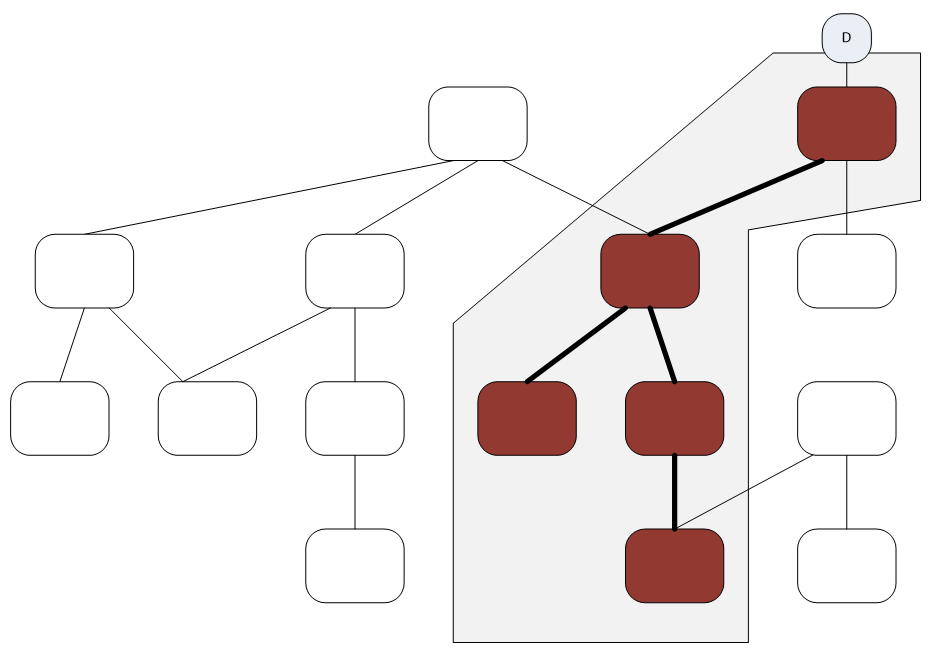
\includegraphics[width=0.7\linewidth]{figs/collaborationTesting.PNG}
\caption{Illustration af Collaboration testing.}
\label{fig:collaborationTesting}
\end{figure}

\paragraph{Fordele ved Collaboration testing}

\begin{itemize}
	\item Intuitivt - Kan følge use cases/user stories.
	\item Specielt brugbart et højniveaus system scope test.
\end{itemize}

\paragraph{Ulemper ved Collaborationp testing}

\begin{itemize}
	\item Testede komponenter testes ikke enkeltvis.
\end{itemize}

%%%%%%%%%%%%%%%%%%%%%%%%%%%%%%%%%%%%%%%%%%%%%%%%%%%%%%%%%%%%%%%%%%%%%%%%%%%%%%%%%%%%%%%%%%%%%%%%%%

\subsubsection{Sandwich testing}

Top-down og Bottom-up kombineres

\begin{figure}
\centering
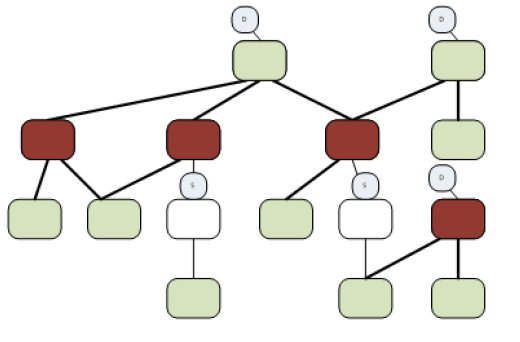
\includegraphics[width=0.7\linewidth]{figs/sandwich.PNG}
\caption{Illustration af Sandwich testing.}
\label{fig:sandwich}
\end{figure}

\paragraph{Fordele ved Sandwich testing}

\begin{itemize}
	\item Man kan bruge både BU og TD hvis det giver mening.
	\item Mange af ulemperne ved BU og TD fjernes - fx det at rpeæsentere low level moduler top-down, bliver lettere hvis nogen af tests er udført i bunden først.
\end{itemize}

\paragraph{Ulemper ved Sandwich testing}

\begin{itemize}
	\item Kræver en stor del planlægning.
\end{itemize}